\documentclass{article}
                            % Useful packages
% Basic page setups
\usepackage[english]{babel}
\usepackage{minted}
\usepackage{ragged2e}
\usepackage{microtype}
\usepackage{hyperref}
\usepackage{tikz}
\usepackage{tikz-3dplot} % for tdplot_main_coords
\hypersetup{
    colorlinks,
    citecolor=black,
    filecolor=black,
    linkcolor=black,
    urlcolor=black
}
\usepackage{mathtools}

\DeclarePairedDelimiter\abs{\lvert}{\rvert}%
\DeclarePairedDelimiter\norm{\lVert}{\rVert}%

% Swap the definition of \abs* and \norm*, so that \abs
% and \norm resizes the size of the brackets, and the 
% starred version does not.
\makeatletter
\let\oldabs\abs
\def\abs{\@ifstar{\oldabs}{\oldabs*}}
%
\let\oldnorm\norm
\def\norm{\@ifstar{\oldnorm}{\oldnorm*}}
\makeatother

\newcommand*{\Value}{\frac{1}{2}x^2}%

\usepackage{listings}
\usepackage{graphicx}
\usepackage{xcolor}
\usepackage[letterpaper,top=2cm,bottom=2cm,left=3cm,right=3cm,marginparwidth=1.75cm]{geometry}
\usepackage[T1]{fontenc} %c<- Times-like font \textcs

% For drawing. i recomend using AI for writing tikz code and then manually edit.
\usepackage{tikz}

% Math
\usepackage{amsmath}
\usepackage{amssymb}
\usepackage{mathabx}
\usepackage{mathptmx}

% For trees
\usepackage[linguistics]{forest}

% For custom symbols [outerjoins]
\def\ojoin{\setbox0=\hbox{$\Join$}%
\rule[0.041ex]{.27em}{.4pt}\llap{\rule[1.032ex]{.27em}{.4pt}}}
\def\leftouterjoin{\mathbin{\ojoin\mkern-6.9mu\Join}}
\def\rightouterjoin{\mathbin{\Join\mkern-6.9mu\ojoin}}
\def\fullouterjoin{\mathbin{\ojoin\mkern-6.9mu\Join\mkern-6.9mu\ojoin}}

% For psudocodes
\usepackage{float}
\usepackage{algorithm}
\usepackage{algorithmicx}
\usepackage[noend]{algpseudocode}
\usepackage{pgfplots}
\pgfplotsset{compat=1.18}
%==================================================================================================================%
\title{Notes for "Calculus"}
\author{Simon Holm\\\\AI503: Calculus\\\\Teacher: Shan Shan}
\date{ }
\begin{document}
\maketitle
\newpage
\tableofcontents
\newpage
\section{Introduktion}
Notes and exercises for lectures and TA-sessions. Note that mistakes in note and/or exercises may occur.
\newpage
\section{Notes}
\subsection{Exercises}

\subsection{Vectors}
\begin{center}
    \begin{tikzpicture}
        \draw[->, thick, blue] (0,0) -- (2,2) node[above] {$\vec{2a}$};
        \draw[->, thick] (0,0) -- (1,1) node[right] {$\vec{a}$};
        \draw[->, thick, red] (0,0) -- (-1,-1) node[below] {$\vec{-a}$};

        % Draw axes
        \draw[->] (0,0) -- (2.5,0) node[right] {$x$};
        \draw[->] (0,0) -- (0,2.5) node[above] {$y$};
        % Add numbers on x-axis
        \foreach \x in {1,2} {
          \draw (\x,0.05) -- (\x,-0.05) node[below] {\x};
        }
        % Add numbers on y-axis
        \foreach \y in {1,2} {
          \draw (0.05,\y) -- (-0.05,\y) node[left] {\y};
        }
    \end{tikzpicture}
\end{center}
What number can you multiply $\vec{-a}$ with to get a vector in the opposite direction?
$$\norm{c\vec{-a}} =c\cdot \sqrt{2}\quad c = \frac{1}{\sqrt{2}}$$

\subsection{Dot Product}
The dot product of two vectors $\vec{a}$ and $\vec{b}$ is defined as:
$$\vec{a} \cdot \vec{b} = \norm{\vec{a}} \norm{\vec{b}} \cos(\theta)$$
where $\theta$ is the angle between the two vectors.
\subsubsection{Example}
Let $$\textbf{v} = \begin{pmatrix} 3 \\ 4 \end{pmatrix}, \quad \textbf{w} = \begin{pmatrix} -4 \\ 3 \end{pmatrix}$$
\begin{itemize}
    \item[1] Compute $\textbf{v} \cdot \textbf{w}$ 
    \item[2] Use (1) to deduce that the angle between $\textbf{v}$ and $\textbf{w}$ is a right angle
    \item[3] Draw the vectors to confirm.
        \subitem Using the definition: 
        \subitem $\textbf{v} \cdot \textbf{w} = \norm{\textbf{v}} \norm{\textbf{w}} \cos(\theta)$
        \subitem $v\cdot w = 25 \cos(0) = 0$
\end{itemize}
\begin{center}
    \begin{tikzpicture}
        \draw[->, thick] (0,0) -- (3,4) node[above] {$\vec{v}$};
        \draw[->, thick] (0,0) -- (-4,3) node[right] {$\vec{w}$};

        % Draw axes
        \draw[->] (0,0) -- (5,0) node[right] {$x$};
        \draw[->] (0,0) -- (0,5) node[above] {$y$};
        % Add numbers on x-axis
        \foreach \x in {1,2,3,4,5} {
          \draw (\x,0.05) -- (\x,-0.05) node[below] {\x};
        }
        % Add numbers on y-axis
        \foreach \y in {1,2,3,4,5} {
          \draw (0.05,\y) -- (-0.05,\y) node[left] {\y};
        }
    \end{tikzpicture}
\end{center}


\newpage

\subsection{Standard Basis Vectors in $\mathbb{R}^3$}
The standard basis vectors in $\mathbb{R}^3$ are:
$$\vec{i} = \begin{pmatrix} 1 \\ 0 \\ 0 \end{pmatrix}, \quad \vec{j} = \begin{pmatrix} 0 \\ 1 \\ 0 \end{pmatrix}, \quad \vec{k} = \begin{pmatrix} 0 \\ 0 \\ 1 \end{pmatrix}$$\\\\

Note that: any vector $\vec{a} = \begin{pmatrix} a_1 \\ a_2 \\ a_3 \end{pmatrix}$ can be written as:
$$\vec{a} = a_1 \vec{i} + a_2 \vec{j} + a_3 \vec{k}$$
\begin{center}
\tdplotsetmaincoords{60}{120} % choose a nice view angle
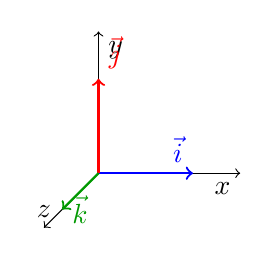
\begin{tikzpicture}[scale=1.2]
    % Axes
    \draw[->] (0,0,0) -- (1.5,0,0) node[anchor=north east]{$x$};
    \draw[->] (0,0,0) -- (0,1.5,0) node[anchor=north west]{$y$};
    \draw[->] (0,0,0) -- (0,0,1.5) node[anchor=south]{$z$};

    % Basis vectors
    \draw[->, thick, blue] (0,0,0) -- (1,0,0) node[anchor=south east]{$\vec{i}$};
    \draw[->, thick, red] (0,0,0) -- (0,1,0) node[anchor=south west]{$\vec{j}$};
    \draw[->, thick, green!60!black] (0,0,0) -- (0,0,1) node[anchor=west]{$\vec{k}$};
\end{tikzpicture}
\end{center}


\subsection{Cross Product}

\subsection{Partial Derivatives}
\subsection{Examples}
Use the second derivative test to classify the critical points of the function
$$f(x,y) = x^3 - 3x + 4.$$

\newpage
\subsection{3dplots}
For the function $$f(x,y) = x^2 + y^2$$
\begin{center}
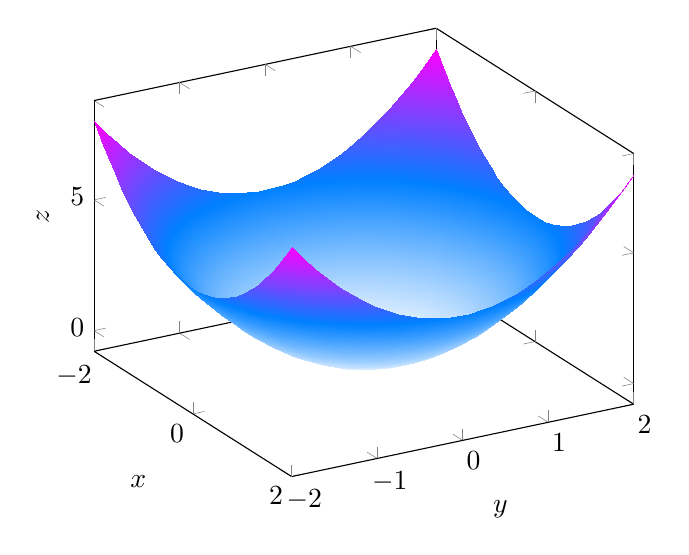
\begin{tikzpicture}
  \begin{axis}[
    view={60}{30},
    domain=-2:2,
    domain y=-2:2,
    samples=30,
    samples y=30,
    xlabel={$x$},
    ylabel={$y$},
    zlabel={$z$},
    colormap/cool,
    mesh/ordering=y varies,
  ]
    \addplot3[surf,shader=interp] {x^2 + y^2};
  \end{axis}
\end{tikzpicture}
\end{center}


For the function $$f(x,z) = x^2 + (z-1)^2$$
\begin{center}
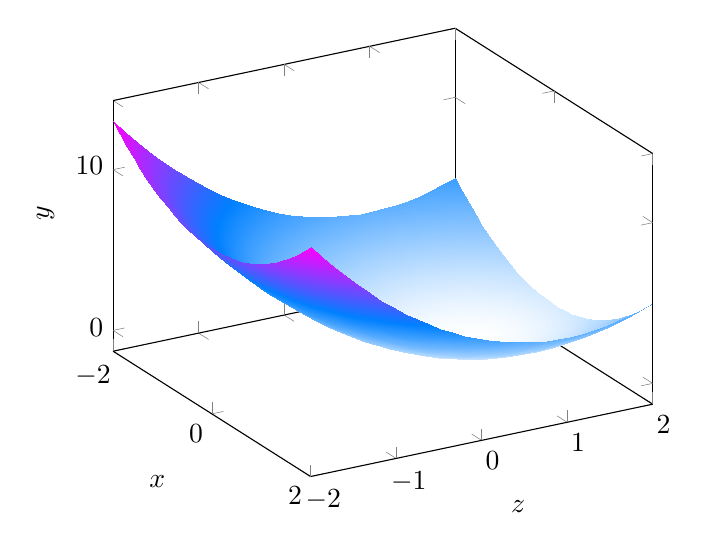
\begin{tikzpicture}
  \begin{axis}[
    view={60}{30},
    domain=-2:2,
    domain y=-2:2,
    samples=30,
    samples y=30,
    xlabel={$x$},
    ylabel={$z$},
    zlabel={$y$},
    colormap/cool,
    mesh/ordering=y varies,
  ]
    \addplot3[surf,shader=interp] {x^2 + (y-1)^2};
  \end{axis}
\end{tikzpicture}
\end{center}

For the function $$f(x,z) = x^2 - z^2$$
\begin{center}
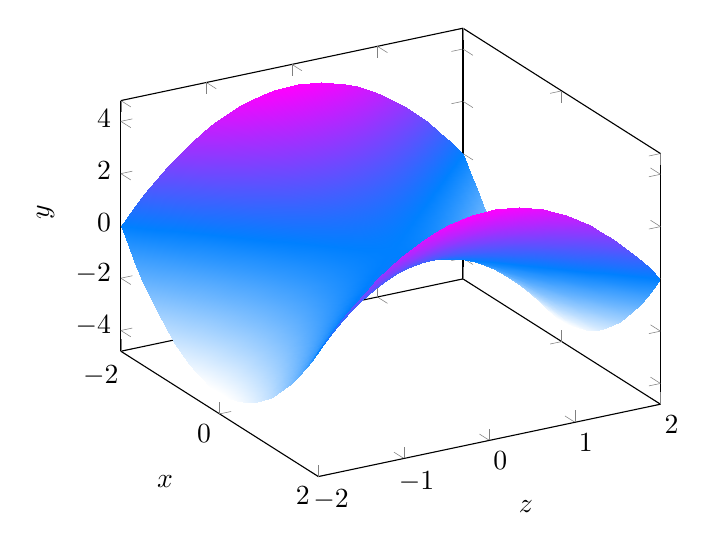
\begin{tikzpicture}
  \begin{axis}[
    view={60}{30},
    domain=-2:2,
    domain y=-2:2,
    samples=30,
    samples y=30,
    xlabel={$x$},
    ylabel={$z$},
    zlabel={$y$},
    colormap/cool,
    mesh/ordering=y varies,
  ]
    \addplot3[surf,shader=interp] {x^2 - y^2};
  \end{axis}
\end{tikzpicture}
\end{center}


\newpage

For the function $$f(x,y) = \sqrt{x^2 + y^2}$$
\begin{center}
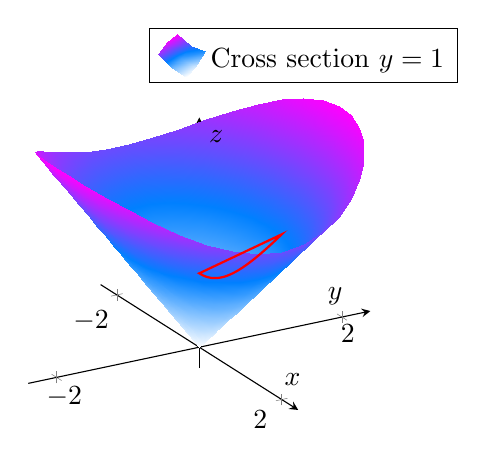
\begin{tikzpicture}
  \begin{axis}[
    view={60}{30},
    domain=0:2,
    domain y=0:360,
    samples=30,
    samples y=40,
    xlabel={$x$},
    ylabel={$y$},
    zlabel={$z$},
    colormap/cool,
    axis lines=middle,
    enlargelimits=true,
    grid=both,
  ]
    % z = sqrt(x^2 + y^2)
    \addplot3[
      surf,
      shader=interp,
      z buffer=sort,
    ]
    ({x*cos(y)},{x*sin(y)},{sqrt(x^2 + (x*sin(y))^2)});

    % Cross section at y=1
    \addplot3[
      thick,
      color=red,
      samples=50,
      domain=0:2,
    ]
    (x,0,{sqrt(x^2 + 1)});
    \addlegendentry{Cross section $y=1$}
  \end{axis}
\end{tikzpicture}
\end{center}

For the function $$f(x,y,z) = \sqrt{x^2 + y^2 + z^2}$$
\begin{center}
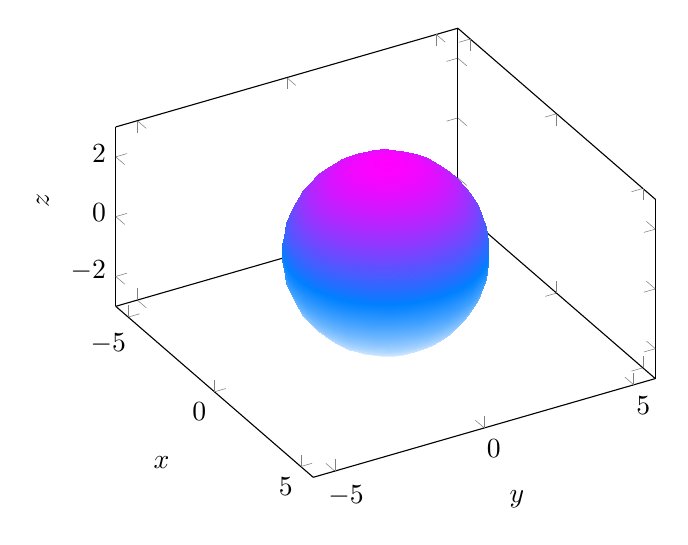
\begin{tikzpicture}
  \begin{axis}[
  view={60}{30},
  domain=0:360,
  domain y=0:180,
  samples=40,
  samples y=20,
  xlabel={$x$},
  ylabel={$y$},
  zlabel={$z$},
  colormap/cool,
  mesh/ordering=y varies,
  axis equal,
  xmin=-3, xmax=3,
  ymin=-3, ymax=3,
  zmin=-3, zmax=3,
  unbounded coords=jump,
  ]
    % Parametric plot of a sphere of radius 2
    \addplot3[
      surf,
      shader=interp,
      z buffer=sort,
    ]
    (
      {3*sin(y)*cos(x)},
      {3*sin(y)*sin(x)},
      {3*cos(y)}
    );
  \end{axis}
\end{tikzpicture}
\end{center}

For the function $$f(x,y,z) = \sqrt{x^2 + y^2 - z^2}$$
\begin{center}
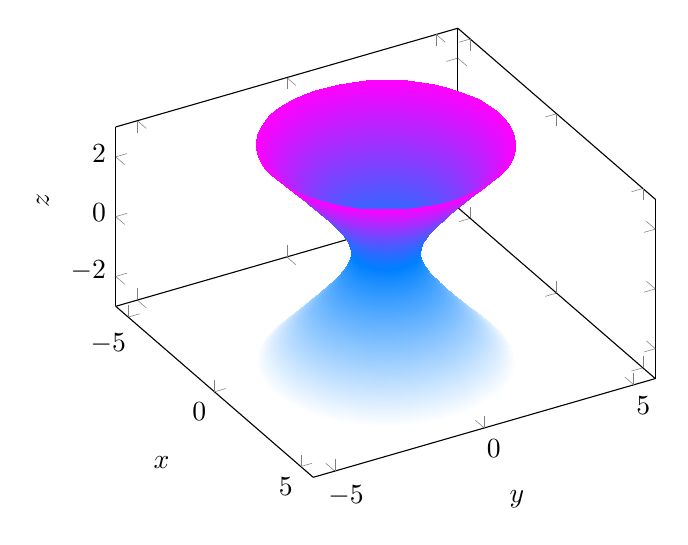
\begin{tikzpicture}
  \begin{axis}[
    view={60}{30},
    domain=0:2*pi,
    domain y=-2:2,
    samples=60,
    samples y=40,
    xlabel={$x$},
    ylabel={$y$},
    zlabel={$z$},
    colormap/cool,
    mesh/ordering=y varies,
    axis equal,
    xmin=-3, xmax=3,
    ymin=-3, ymax=3,
    zmin=-3, zmax=3,
    unbounded coords=jump,
  ]
    % Parametric plot of the hyperboloid x^2 + y^2 - z^2 = 1
    \addplot3[
      surf,
      shader=interp,
      z buffer=sort,
    ]
    (
      {cosh(y)*cos(deg(x))},
      {cosh(y)*sin(deg(x))},
      {sinh(y)}
    );
  \end{axis}
\end{tikzpicture}
\end{center}

\end{document}
